\section{Benutzerschnittstelle}
	In diesem Abschnitt dieses Kapitels wird auf die Umsetzung der Benutzerschnittstelle eingegangen. Wie schon bereits im SRS erwähnt handelt es sich bei der Benutzerschnittstelle um die grafische Oberfläche der Anwendung. Dafür wird zunächst auf die Umsetzung der verschiedenen UI Elemente eingegangen sowie relevante Funktionalitäten beschrieben. Abschließend wird die Evaluation des Usability Tests behandelt. 
		
	\subsection{Benutzeroberfläche}	
		Die Implementierung der Benutzeroberfläche ist von Anfang der Umsetzungsphase bis zum Ende ein kontinuierlicher, iterativer und wichtiger Entwicklungsprozess. Es beginnt mit einer ganz simplen Steuerung zum Testen von Funktionen bis zum Perfektionieren aller benötigter User Interface Elemente. Als erstes werden die Startbildschirme und der Registrierungsprozess behandelt. 
		
		\subsubsection{Startbildschirm und Registrierung}
			Das aller erste, was der Spieler von NoRPG sieht und womit er interagieren darf, ist der Startbildschirm. Dieser ist besonders wichtig, da hier die ersten Eindrücke schon gesammelt werden. Bei dem Startbildschirm wird zwischen zwei Varianten unterschieden. In der ersten Variante startet der Spieler NoRPG das erste mal oder ist nicht mit seinem Account angemeldet. In der zweiten Variante ist der Benutzer schon angemeldet. Diese beide Varianten sind in der Grafik \ref{startScreenUI} dargestellt.
			
			\begin{figure}[htbp]
				\centering 
				\label{startScreenUI}
				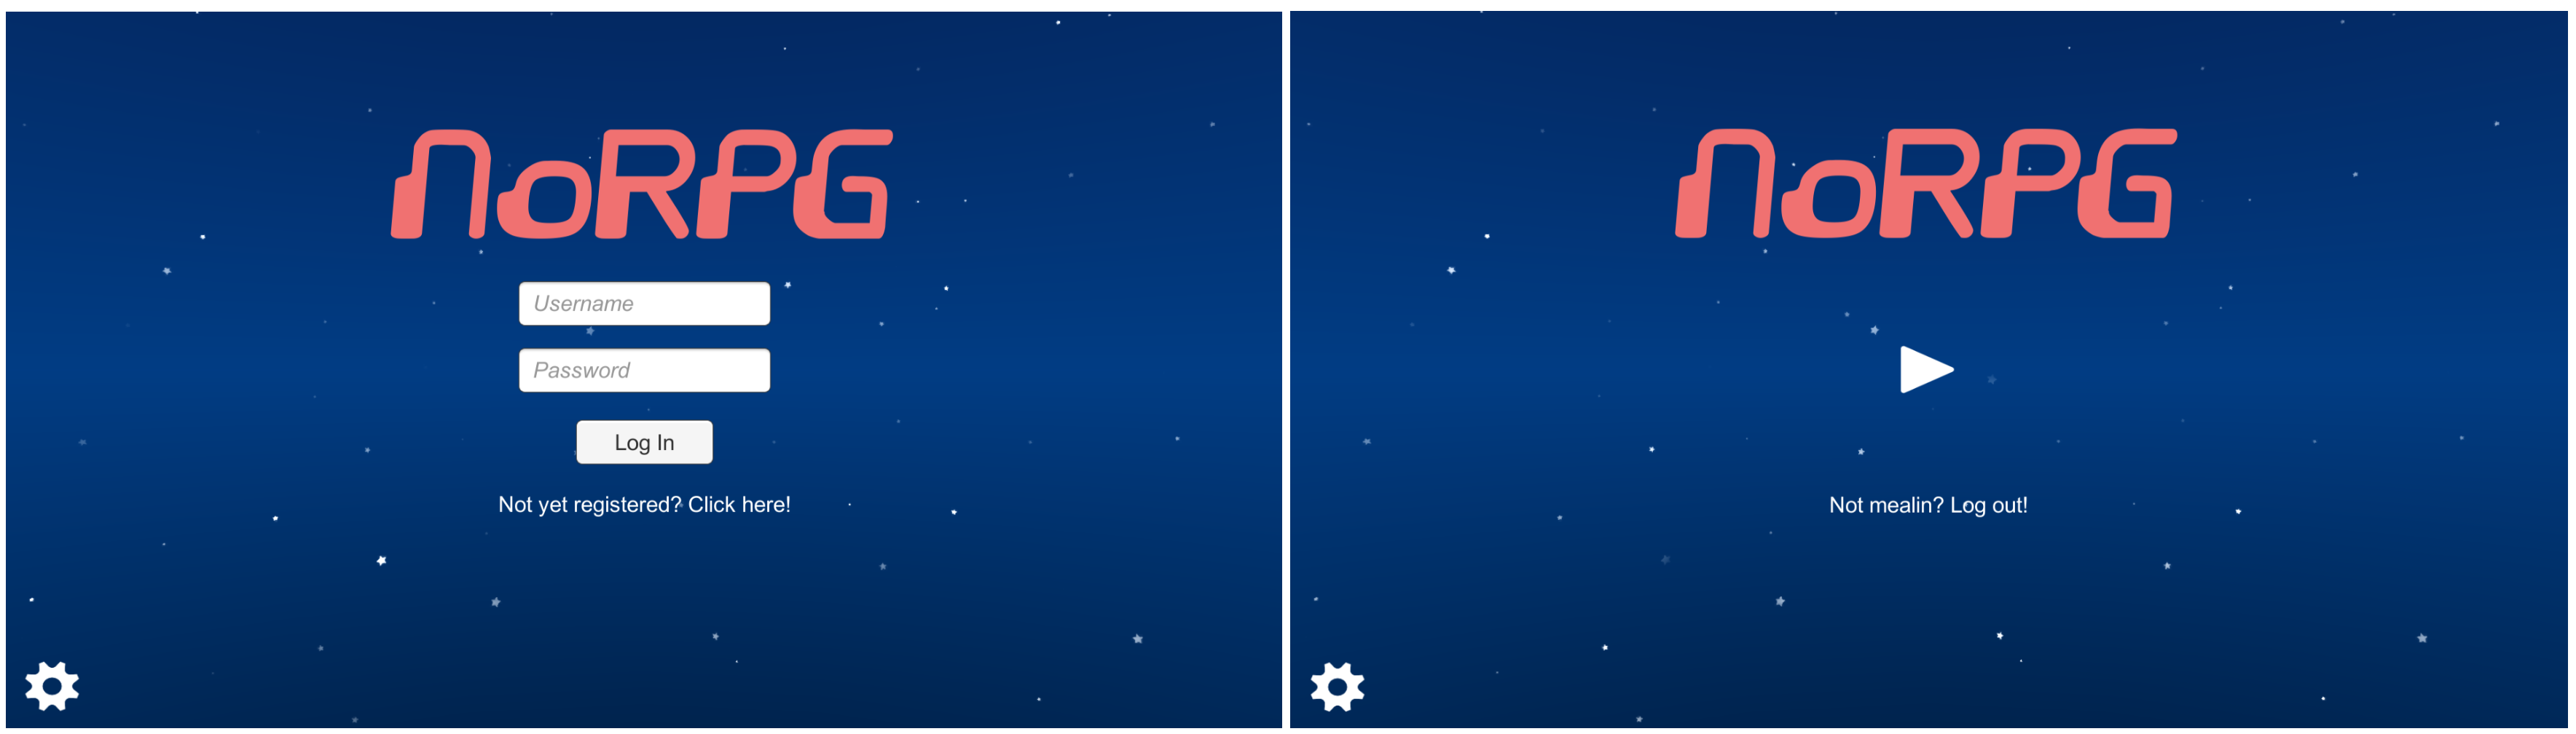
\includegraphics[width=\textwidth]{pics/startbildschirmeScreen.png}
				\caption{User Interface: Startbildschirm}
			\end{figure}
			
			Beide Varianten ähneln sich nicht nur im aussehen sondern auch in der Implementierung. Die Startbildschirme wurden nach dem Gestaltungsprinzip Figure/Ground entworfen und umgesetzt. Figure/Ground unterteilt die Wahrnehmung visueller Informationen in Figure (Vordergrund) und Ground (Hintergrund). Dabei liegt der Fokus auf dem Vordergrund. Das Design und Aussehen der Komponenten ist dabei Clean und Simple, zu Deutsch sauber und einfach. Dieter Rams beschreibt in seinem Buch "Weniger, aber besser / Less but better" \cite{ramsDesign}, dass einfaches Design nicht über die Subtraktion von Dingen von einem Design handelt, sondern die Gesamteffektivität des Designs zu verbessern. Elemente in der Benutzeroberfläche haben so wenig Text und Farbe wie notwendig und werden, falls möglich, nur mit Symbole abgebildet. Dabei wird ein intuitives Design verwendet, welches die Spieler wahrscheinlich aus anderen Spielen schon kennen und nicht neu lernen müssen.
			
			Der Vordergrund von beiden Varianten ist in zwei Abschnitte unterteilt. Der erste Abschnitt ist in der Mitte des Bildschirm positioniert und bindet die Aufmerksamkeit des Spielers. In der ersten Variante besteht dieser aus zwei Eingabefelder für die Benutzerdaten, dem Log-In Button und einem Textfeld, um sich zu registrieren. In der zweiten Variante allerdings besteht dieser Abschnitt nur aus einem Button zum Starten des Spieles und einem Textfeld für die Abmeldung. Der zweite Abschnitt ist an der unteren Seite des Bildes positioniert und besteht aus einem Button für die Einstellungen. Dabei öffnet sich kein Fenster, sondern werden Symbole für die Einstellungsmöglichkeiten ein- und ausgeblendet.
			
			Der Hintergrund setzt sich aus dem Logo und einem Sternenhimmel zusammen. Diese Hintergrundelemente sind 3D-Elemente, welche in der Spielwelt angebracht sind und durch eine Kamera aufgezeichnet werden. Neben diesen Hintergrundelementen gibt es ein weiteres Element, welches erst durch die Betätigung des Log-In Buttons auftaucht. Es handelt sich um ein drehendes Icon, dass den Ladeprozess darstellt und somit dem Spieler ein Feedback gibt. Der Hintergrund ist sehr schlicht aber farbenfroh gestaltet. Zudem sind die Sterne am Himmel animiert, welches einen besonders positiven Eindruck hinterlassen soll.
			
			Die Startbildschirme sind mit dem Standard Render-Modus Screen Space - Overlay umgesetzt worden. Dieser Modus unterstützt das Gestaltungsprinzip Figure/Ground, indem die UI Elemente vor den Hintergrund gerendert werden. Fernerhin kann der Spieler sich innerhalb des Startbildschirm nicht bewegen oder andere Interaktionen ausführen, sodass ein anderer Render-Modus notwendig wäre.

			Auf Grund der Tatsache das es zwei Startbildschirme gibt, muss bevor der anzuzeigende Startbildschirm angezeigt wird eine Überprüfung stattfinden. Die aller erste Szene die in NoRPG geladen wird, ist eine nahezu leere Szene, die nur aus dem Hintergrund, einem kleinen Textfeld und einem Skript besteht. Diese Szene ist deshalb so minimalistisch gestaltet, damit das Laden und somit das Ausführen des Skriptes sehr schnell durchgeführt werden kann, so dass der Spieler im besten Fall diese Szene erst gar nicht sieht und bemerkt. Das Skript prüft, ob die in Kapitel 5.1 beschriebene lokale Datei, mit den Informationen über den Spielstand des Spielers, vorhanden und vollständig ist. Ist dies der Fall, kann davon ausgegangen werden, dass der Spieler angemeldet ist und die zweite Variante des Startbildschirmes wird geladen. Der Hintergrund ist notwendig, falls das Laden länger braucht der Spieler keinen weißen beziehungsweise leeren Hintergrund sieht. Das Textfeld in dieser Szene ist angebracht, damit der Spieler im Fehlerfall informiert wird.
			
			Die nächste Benutzeroberfläche, die behandelt wird, ist die Registrierung. Ein Teil des Registrierungsprozesses ist in Abbildung \ref{registerUI} abgebildet.
			
			\begin{figure}[htbp]
				\centering 
				\label{registerUI}
				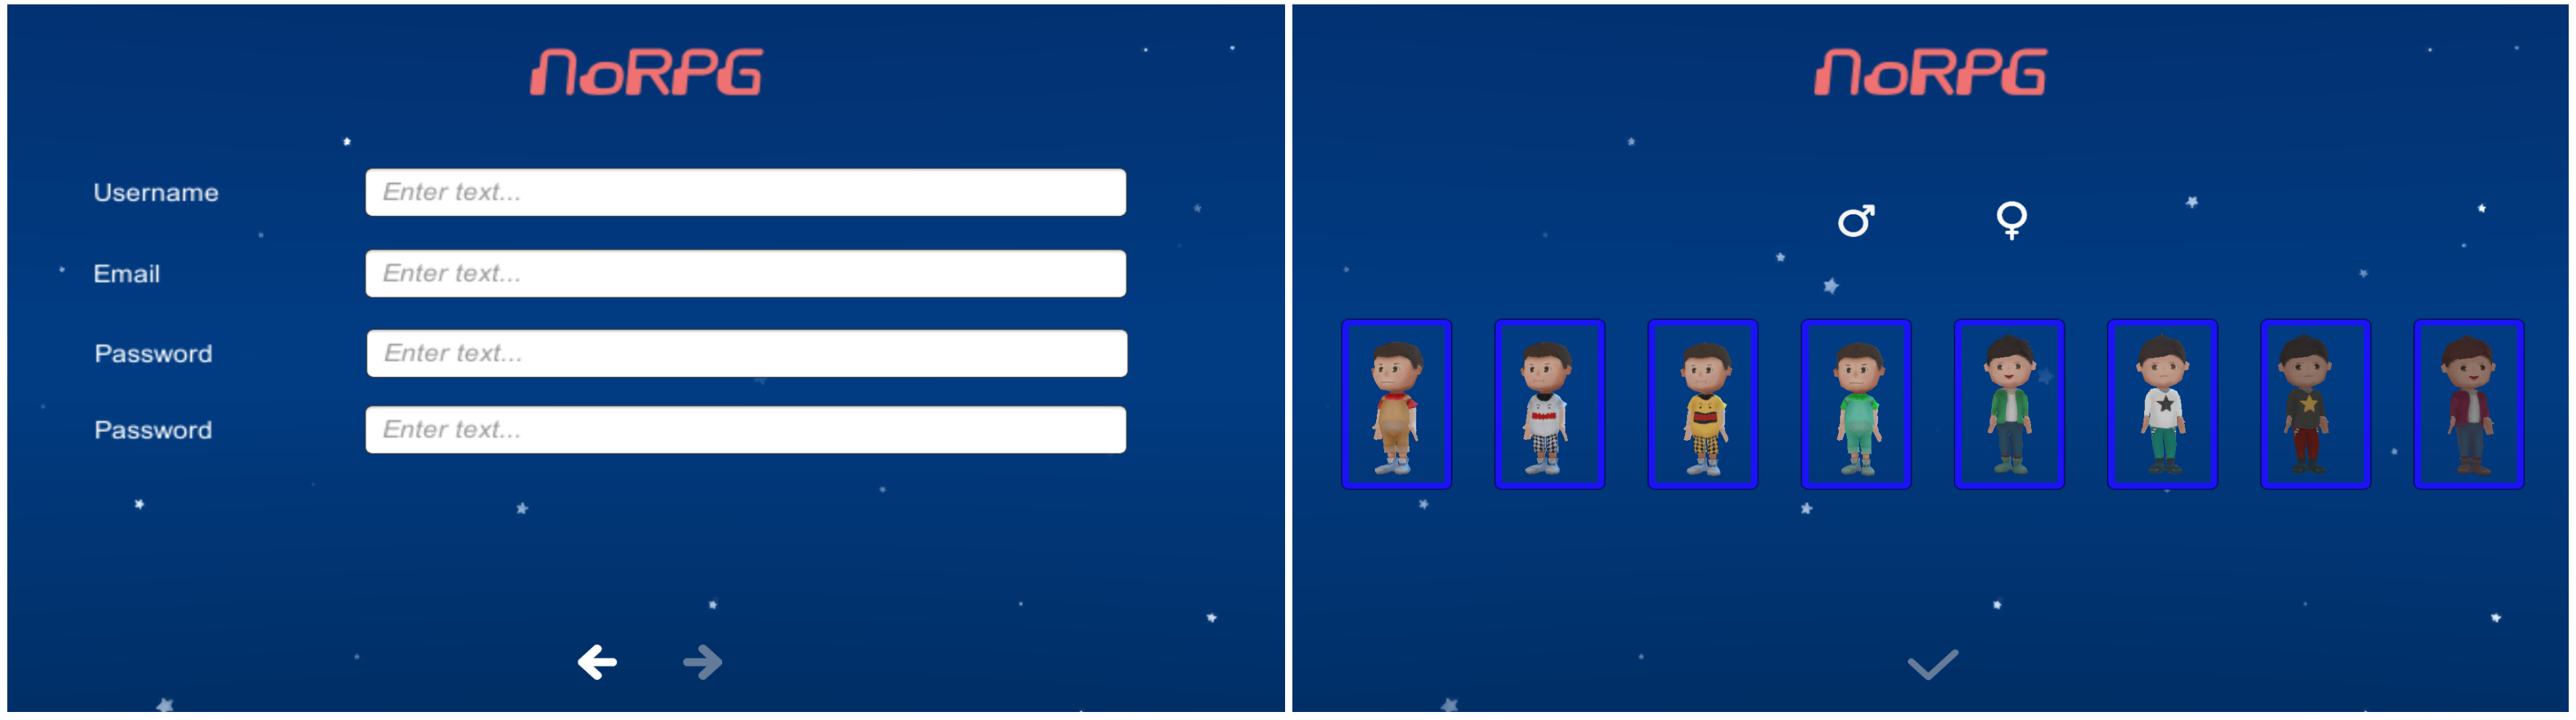
\includegraphics[width=\textwidth]{pics/registerScreen.png}
				\caption{User Interface: Registrierung}
			\end{figure}
		
			Es fällt auf, dass auch hier das Gestaltungsprinzip Ground/Figure umgesetzt wurde. Dies hat die gleichen Gründe wie bei den Startbildschirmen und die Konsistenz außerhalb des eigentlichen Spieles bleibt erhalten. Neben diesen Gestaltungsprinzip wurde versucht das Prinzip Simple und Clean weiter fortzuführen, allerdings handelt es sich bei der Registrierung um einen komplexeren Prozess. Daher wurde ein weiteres Gestaltungsprinzip verwendet. Die UI Elemente sind tabellarisch angeordnet und deren relative Abstände gruppieren einzelne Elemente. Dieses Prinzip wird Proximity genannt. Dadurch weiß der Spieler welche Eingabefelder zu welchen Textfeldern gehören und kann somit die korrekten Informationen angeben. Auch hier ist das User Interface in zwei Abschnitte unterteilt. Der erste Abschnitt ist in der Mitte des Bildschirms positioniert und bildet das Registrierungsformular ab. Der zweite Abschnitt ist am unteren Teil des Bildes und dient zur Navigation durch den gesamten Registrierungsprozess.
			
			Der größte Unterschied ist allerdings, dass diese Szene mit dem Render-Modus World Space implementiert wurde. Der letzte Schritt im Registrierungsprozess ist die Auswahl des Charakters. Damit die einzelnen Charaktere in die UI integriert werden konnten, musste dieser Modus umgesetzt werden. Dadurch wurde möglich, dass zunächst die 3D Objekte der Welt nicht von den UI Elementen verdeckt werden und anschließend kann der Spieler auf seinen gewünschten Charakter klicken und es wird eine Animation ausgeführt. 
		
		\subsubsection{Head-Up Display im Spiel}
			Das Head-Up Display bildet das User Interface innerhalb des Spieles ab. Grundsätzlich kann das HUD in vier Abschnitte unterteilt werden. Die Abschnitte sind an den Ecken des Bildschirmes positioniert. Diese Positionierung hat den Vorteil, dass die UI Elemente nicht vom Spiel ablenken und Informationen verdecken, sowie der Spieler die Elemente einfach mit den Händen erreichen kann. Abbildung \ref{alwaysOnUI} stellt die standardmäßige Ansicht von NoRPG dar.
			
			\begin{figure}[htbp]
				\centering 
				\label{alwaysOnUI}
				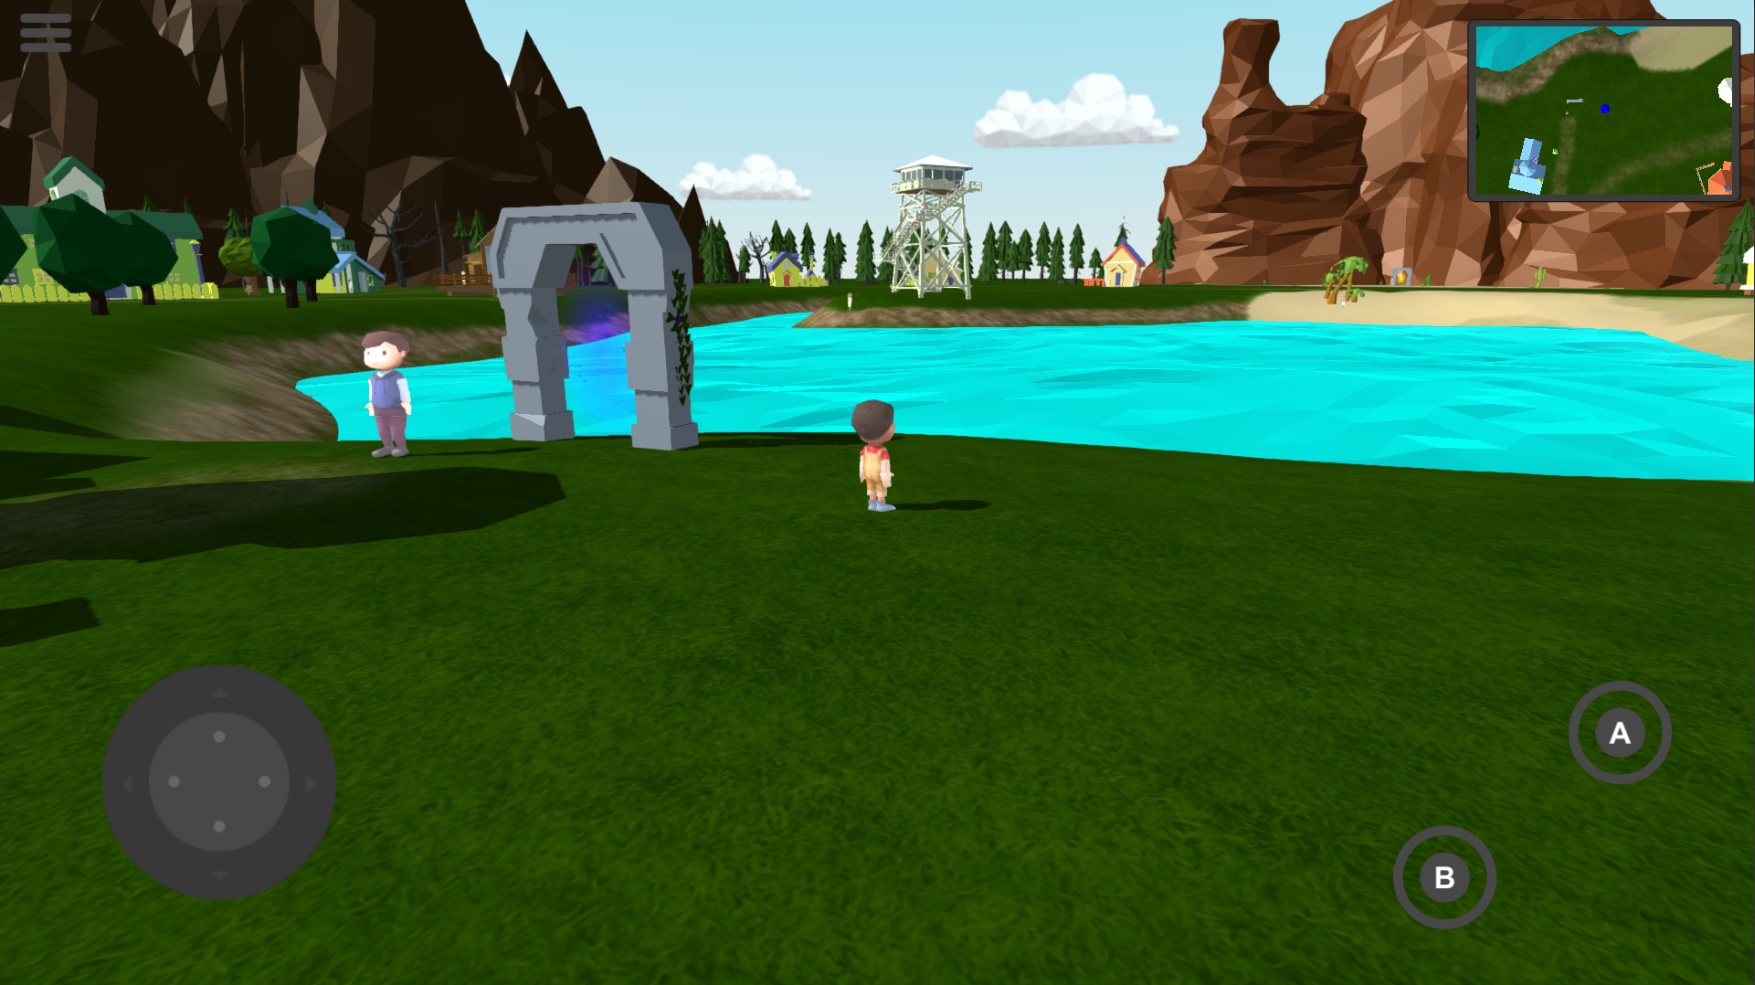
\includegraphics[width=13cm]{pics/alwaysOnUI.png}
				\caption{User Interface: Head-Up Display}
			\end{figure}
		
			Das ganze HUD ist mit dem Render Modus Screen Space - Overlay implementiert. Das HUD steht nicht im Fokus, darf allerdings nicht durch 3D Objekte verdeckt werden. Die HUD Elemente dienen zur Steuerung des Spieles und sind genauso wichtig wie das Spiel selber.
			
			\paragraph{Der Joystick}
				Der Joystick befindet sich in der unteren linken Ecke. Der Spieler kann mit Hilfe des Joysticks sich im Spiel fortbewegen. Von allen UI Elementen die NoRPG implementiert wurden, ist der Joystick das einzige Elemente, das nicht standardmäßig von Unity zur Verfügung stellt. Bei dem Joystick handelt es sich um ein Asset, welches aus dem Unity Asset Store erworben wurde. Die Besonderheit ist, dass der Joystick aus drei Elementen besteht, welche übereinander liegen. 
				
				Das oberste Element ist der sogenannte Stick. In der Abbildung \ref{alwaysOnUI} handelt es sich um kreisförmige hellgraue Element in der linken Ecke. Der Spieler interagiert mit dem Stick und kann diesen in alle Richtungen bewegen. Diese Bewegungen werden dann anschließend mit Einsatz eines Skriptes an den Charakter im Spiel übergeben. 
				
				Bei dem zweiten Element handelt es sich um die Basis des Joysticks. Bei Bewegungseingaben des Spielers ändert sich die Position nicht. Die Basis dient zum einen der Orientierung und begrenzt den Radius des Sticks. Je nachdem wie weit außerhalb der Stick sich innerhalb dieses Radius befindet, bewegt sich der Charakter mit einer unterschiedlichen Geschwindigkeit.
				
				Das unterste Elemente wird als Touch Zone bezeichnet. Diese ermöglicht innerhalb eines festgelegten Bereiches, dass der Spieler seinen Daumen in eine beliebige Position setzen kann und der Joystick wird genau unter seinem Daumen platziert. Dadurch wird gewährleistet, dass junge Spieler, die eher kleinere Hände haben, und Erwachsene komfortabel den Joystick verwenden können.
				
			\paragraph{Die Interaktionbuttons}
				Bei den Interaktionsbuttons handelt es sich um die Buttons, die für die Steuerung der Interaktionen in NoRPG zuständig sind. Diese sind an der unteren rechten Ecke positioniert. Es wird zwischen zwei Buttons mit unterschiedlichen Zuständigkeiten unterschiedenen. Der rechte Button, der A-Button, ist für das Starten einer Interaktion und für das Akzeptieren bei Entscheidungsfällen verantwortlich. Der zweite Button, der B-Button, wird zum Abbrechen von Interaktionen benötigt. Allerdings gibt es Situationen, in denen beide Buttons die gleiche Funktionalität abbilden, beispielsweise am Ende einer Konversation kann der Spieler mit beiden Buttons diese beenden. Eine Konversation ist in Abbildung \ref{userInterfaces} im oberen linken Teil abgebildet.
				
				Damit jedoch nicht immer irgendeine Interaktion gestartet wird, wenn der Spieler die Taste verwendet, wurde ein Skript implementiert, der den Abstand vom Spieler zum nächsten Objekt im Spiel bestimmt. Erst wenn der Spieler sich in der Nähe des Objektes befindet, wird eine Interaktion gestartet.
				
				Bei den Buttons handelt es sich um standardmäßige Buttons von Unity. Allerdings sind diese mit einer animierbaren Textur überzogen. Die Textur verändert das aussehen des Buttons und ermöglicht visuelles Feedback zurückzugeben, falls der Button geklickt wird oder für einen Moment nicht benutzbar ist.
				
				\begin{figure}[htbp]
					\centering 
					\label{userInterfaces}
					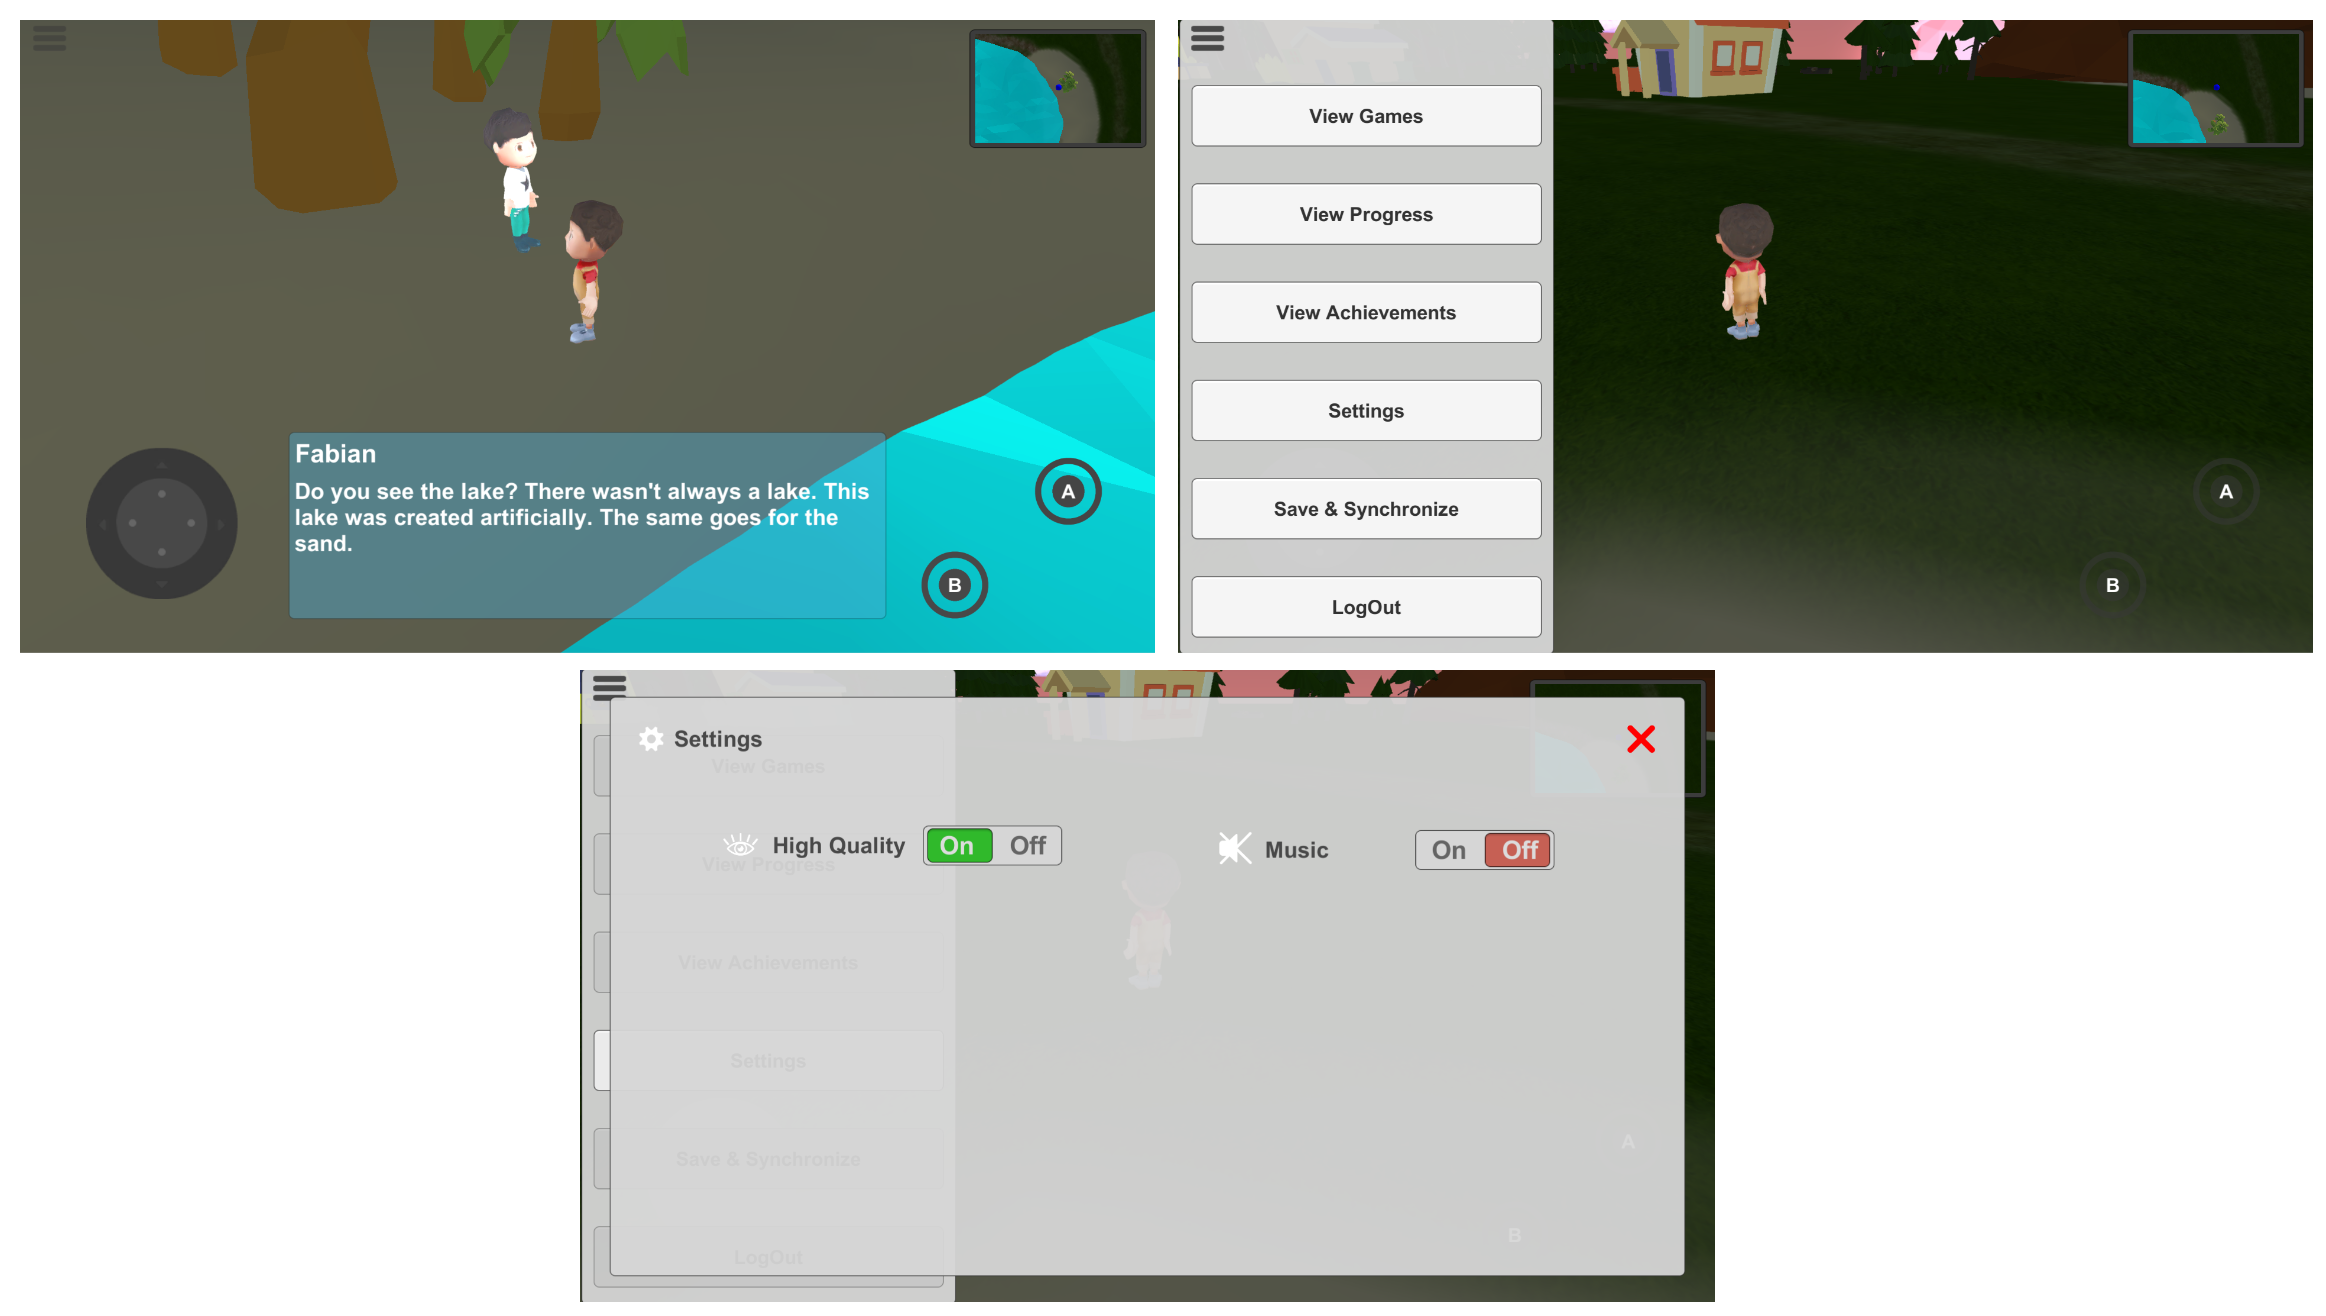
\includegraphics[width=\textwidth]{pics/userInterface.png}
					\caption{User Interfaces: Kommunikation, Menu und Einstellungen-Fenster}
				\end{figure}
			
			\paragraph{Das Menü}
				Der Button für das Menü befindet sich in der oberen linken Ecke. Dieser ist im oberen Teil des Bildschirms positioniert, da die Häufigkeit der Benutzung wesentlich geringer ist, als bei den bisher besprochenen UI Elementen.
				
				Bei der Verwendung des Buttons öffnet sich das Menü im linken Teil des Bildschirms. Dies im unteren linken Bild der Abbildung \ref{userInterfaces} abgebildet. Das geöffnete Fenster beinhaltet alle restlichen Funktionen, die nicht direkt über das HUD erreicht werden können. Beispielsweise findet der Spieler die Einstellungen oder kann seinen Fortschritt öffnen. Diese Funktionen sind in dem Menü, da die Informationen nicht immer benötigt werden und deshalb nicht die ganze Zeit sichtbar sein müssen. Während das Menü offen ist können keine anderen UI Elemente, wie die Buttons zur Interaktion verwendet werden. Der Spieler muss erst das Menü schließen um wieder mit dem Spiel fortfahren zu können. 
				
				Es wird zwischen zwei Varianten von Funktionen im Menü unterschieden. Einige der Funktionen öffnen ein weiteres Fenster, wie in der Abbildung \ref{userInterfaces} im unteren rechten Bild abgebildet, und andere werden direkt im Menü ausgeführt. So wird beispielsweise für die Einstellungen ein weiteres Fenster geöffnet, wohingegen das Speichern direkt im Menü durchgeführt wird, ohne das sich ein Fenster öffnet.
			
			\paragraph{Die Karte}
				Die Karte im oberen rechten Eck des Bildschirms wird als Mini Map bezeichnet. Sie bietet dem Spieler einen Überblick über seine aktuelle Position. Realisiert wurde diese Mini Map mit einer zusätzlichen zweiten Kamera, die von oben auf den Spieler schaut. Das Objekt der Mini Map ist am Charakter angebracht, damit der Spieler und die Mini Map sich immer in der gleichen Position befinden.
								
				Da zwei Kameras die Komplexität der Szene erhöhen, indem alle Bilder doppelt dargestellt werden, muss die zusätzliche Kamera angepasst werden. Diese rendert die Szene nicht mit der gleichen Qualität wie die Hauptkamera. Des Weiteren werden einige Elemente, wie beispielsweise Schatten oder zu kleine 3D-Objekte wie Blumen nicht in der Mini Map gerendert. 
				
				Der Spieler kann auf die Mini Map klicken und es wird die komplette Karte der aktuellen Spielwelt geöffnet. Diese Übersicht wird ebenfalls mit einer Kamera aufgenommen. Der Unterschied allerdings ist, dass diese Kamera nur eingeschaltet ist, also nur dann rendert wenn der Spieler auf die Mini Map klickt. Die Karte kann in Abbildung \ref{userInterfaces} im oberen rechten Bild betrachtet werden.
				
				Die Kamera ist nicht wie die Mini Map am Spieler angebracht, sondern schwebt über der ganzen Szene. Die Karte zeigt ebenfalls keine Schatten oder zu kleine Objekte an, wodurch Ressourcen gespart werden.
				
				Während die Karte offen ist kann der Spieler nicht das Menü öffnen oder eine Interaktion starten, allerdings kann sich der Spieler mit dem Joystick bewegen. Die Kamera dient zur Orientierung in der Spielwelt, deshalb darf der Spieler sich bewegen. Die Karte kann während dem Laufen geöffnet und geschlossen werden.
			
	\subsection{Usability Evaluation}
		Ein Usability Test wird durchgeführt, um die Gebrauchstauglichkeit einer Software oder Hardware mit den potenziellen Benutzern zu überprüfen. Usability wird durch die Attribute Erlernbarkeit, Effizienz, Einprägsamkeit, Fehlerrate und Zufriedenheit\footnote{Vgl. Nielsen \cite{NielsenUI} Seite 26} beschrieben. Unter dem Attribut Erlernbarkeit beschreibt Nielsen in seinem Buch, dass die Anwendung leicht zu erlernen sein muss, damit der Benutzer in kurzer Zeit beginnen kann das Spiel zu spielen. Dazu zählt beispielsweise die Steuerung. Diese ist wichtig, damit der Benutzer sich im Spiel intuitiv bewegen kann. So bald der Spieler das System gelernt und verstanden hat, soll ein hohes Maß an Produktivität möglich sein. Dies wird als Effizienz bezeichnet. Das System sollte allerdings leicht zu merken und einprägsam sein, so dass auch der Gelegenheitsbenutzer in der Lage ist, nach einer gewissen Zeit ohne Verwendung der Anwendung, in das Spiel zurückzukehren, ohne alles nochmals neu lernen zu müssen. Nielsen weißt zudem darauf hin, dass Fehler für den Benutzer sehr frustrierend sein können. Daher sollte das System eine geringe Fehlerquote haben, so dass Benutzer bei der Verwendung nur wenig Fehler machen und falls Probleme auftauchen, diese den Spaß am Spielen nicht einschränken\footnote{Vgl. Nielsen \cite{NielsenUI} Seite 27ff.}. Das letzte Attribut beschreibt den Gesamteindruck.
		
		Es wird zwischen formativem und summativem Usability Test unterschieden. Foramtive Tests werden während der Entwicklung durchgeführt. Die Aufgabe ist es ein spezielles Problem bzw. Szenario zu testen. Es handelt sich dabei um eine kleine Studie für schnelles Feedback, welche wiederholt durchgeführt werden kann\footnote{Vgl. Rubin und Chisnell \cite{handbookUsability} Seite 29f.}. Der summative Test findet einmalig nach der Entwicklung statt, bevor das fertige Produkt ausgeliefert wird. Dabei handelt es sich um eine umfangreiche Studie, die alle Funktionen der Benutzeroberfläche bewertet\footnote{Vgl. Rubin und Chisnell \cite{handbookUsability} Seite 34f.}.
		
		Ein Usabilty Test kann in verschiedenen Testumgebungen durchgeführt werden. Es wird zwischen Labortest, Feldtest und Remotetest unterschieden. Bei einem Labortest handelt es sich entweder um ein Usability Labor oder um einen allgemein nutzbaren Raum. Der ausschlaggebende Unterschied zwischen diesen beiden ist, dass das Usability Labor nur für Usabilty Tests und Evaluationen verwendet wird. Die potenziellen Tester werden eingeladen und führen die Auswertung in diesem Raum durch. Zu den Basisutensilien gehört neben Nahrung und Verpflegung die notwendige Hardware und Software, sowie ein Moderator bzw. Experte für Fragen und Probleme\footnote{Vgl. Rubin und Chisnell \cite{handbookUsability} Seite 101f.}. Der Feldtest oder auch Mobiler Test kann potentiell überall durchgeführt werden, sei es beim Kunden, in einem öffentlichen Gebäude oder in einem Café. Der Vorteil im Vergleich zu einem Labortest ist, dass der Benutzer sich einer gewohnten und reale Umgebung mit echten Lichtverhältnissen befindet. Allerdings ist es wahrscheinlicher das der Tester durch die Umwelt abgelenkt wird\footnote{Vgl. Rubin und Chisnell \cite{handbookUsability} Seite 98f.} und der Experte mit zum Kunden. Bei der letzten Möglichkeit ist der Benutzer und Moderator örtlich voneinander getrennt. Der Remotetest kann synchron, indem der Moderator und die Teilnehmer per Audio- oder Videokonferenz verbunden sind, oder asynchron stattfinden. Der wesentliche Vorteil ist, dass dadurch potenziell mehr Testpersonen teilnehmen und es günstiger ist. Allerdings können keine komplexen Anforderungen gestellt werden und bei Fragen ist der Tester mehr oder weniger auf sich gestellt.
		
		\subsubsection{Vorbereitung und Durchführung}
			Bei der in diesem Kapitel beschrieben Evaluation handelt es sich um einen summativen Remotetest. Der Usability Test findet erst nach der Entwicklung von NoRPG statt und nachdem alle Funktionen implementiert wurden. Die Gründe für einen Remotetest sind, da eine es sich bei NoRPG um eine mobile Anwendung handelt und diese am besten auf dem eigenen Smartphone getestet werden kann. Dadurch werden auch verschiedenste Hardware und Android Versionen geprüft und validiert. Ein weiterer essentieller Punkt sind die Kosten. In dem Umfang dieser Studienarbeit ist es nicht möglich ein Feldtest oder Labortest durchzuführen.
	
			In der Vorbereitung des Usability Tests gilt es zunächst die Benutzerprofile zu erstellen, die zu testenden Szenarien und Ziele, sowie den Umfang zu definieren. Anschließend die Unterlagen vorzubereiten, die Teilnehmer zu rekrutieren und den Zeitraum festzulegen. Das Profil für die Tester ist das gleiche wie das der potenziellen Spieler. Daher wird kein festes Profil für die Evaluation festgelegt, da NoRPG für jung oder alt und männlich oder weiblich ausgelegt ist. Jedoch gilt bei der Rekrutierung zu beachten, das von jeder Alters- und Geschlechtsgruppe eine gewisse Anzahl vertreten ist.
		
			Das Ziel dieser Evaluation ist das Testen der Benutzeroberfläche, da es sich bei einer mobilen Anwendung um die einzige Interaktionsschnittstelle für die Benutzer handelt. Aus diesem Grund ist eine fehlerfreie, intuitive und gleichzeitig gut aussehende Benutzeroberfläche sehr wichtig. Zu den abzubildenden Szenarios gehört zum Beispiel die Registrierung, der Log-In oder die Liste der heruntergeladenen Spiele. Alle User Interface Elemente sollen in diesem summativen Test geprüft und evaluiert werden und aus diesem Grund ist der Umfang dieser Evaluation größer. Diese findet in dem Zeitraum 24.04.2017 bis 30.04.2017 statt.
		
<<<<<<< HEAD
			Für die Evaluation wurde ein Dokument für die Tester erstellt. Dieses beinhaltet alle notwendigen Information und ist zugleich eine Schrittanleitung, um alle UI Elemente testen zu können. Ein ausgefülltes Formular\ref{ueMarcel}, dessen Publikation von dem Tester genehmigt wurde, befindet sich im Anhang dieser Arbeit. Neben den Informationen gibt es mehrere Spalten, die für die Bewertung dienen. Bewertet werden kann ein Szenario mit "++", "+", "0", "\-" und "\--". 
=======
			Für die Evaluation wurde ein Dokument für die Tester erstellt. Dieses beinhaltet alle notwendigen Information und ist zugleich eine Schrittanleitung, um alle UI Elemente testen zu können. Ein ausgefülltes Formular\ref{ueMarcel}, dessen Publikation von dem Tester genehmigt wurde, befindet sich im Anhang dieser Arbeit. Neben den Informationen gibt es mehrere Spalten, die für die Bewertung dienen. 
>>>>>>> 8fe80366cb856ab7f4813d238513c206cb6929ef
		
		\subsubsection{Bewertung}
			Für die Evaluation von NoRPG wurde an alle potenzielle Tester eine Prerelease Version der App und der auszufüllende Bewertungsbogen verteilt. Weitere Anweisungen wurden nicht mitgeteilt.
			
			Zunächst werden alle zusätzlichen Informationen, die aus den Fragebögen gewonnen werden konnten, behandelt und deren Verteilung betrachtet.
			
			Bei dem durchschnittlichen Tester handelt es sich um einen 19 Jahre alten männlichen Tester aus Deutschland. Diese Aussage beruht auf der Auswertung des Fragebogens, welche in Abbildung \ref{auswertungTester} abgebildet sind. Von allen teilnehmenden Testern sind davon 81\% männlich und die übrigen 19\% weiblich. Für die Auswertung wurden drei Altersgruppen definiert und festgelegt. Die meisten Teilnehmern waren über 20 Jahre, da eine Evaluation von Kindern alleine schwer ausgefüllt werden kann. Die jüngeren Tester haben mit Hilfe einer Aufsichtsperson NoRPG getestet und das Ergebnis in der Evaluation festgehalten. Der Großteil der Tester kommt aus Deutschland, allerdings ergab sich die Möglichkeit, einige Tester aus der Türkei zu gewinnen. Diese Erkenntnisse haben Einfluss und Bedeutung in der Bewertung von NoRPG.
			
			\begin{figure}[htbp]
				\centering 
				\label{auswertungTester}
				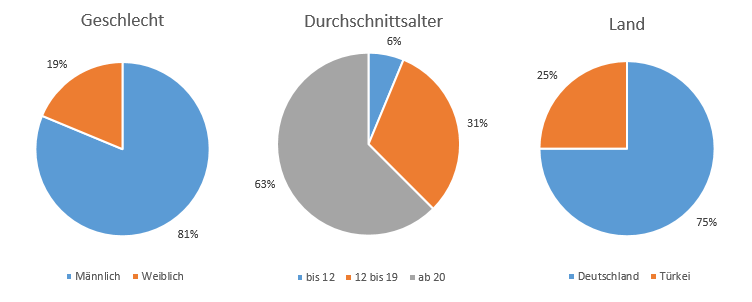
\includegraphics[width=\textwidth]{pics/TesterAuswertung.png}
				\caption{Evaluation Auswertung - Der durchschnittliche Teste}
			\end{figure}
			
			Neben dem Alter, Geschlecht und Herkunftsland konnten die Tester zudem auch die Marke des Smartphone-Herstellers und die installierte Android Version angeben. Dies hat den Zweck, ob die Einschränkungen im SRS im Vorhinein korrekt und sinnvoll waren. Das Ergebnis ist in der Abbildung \ref{auswertungSmartphones} zu sehen. Mit einem Anteil von 50\% ist die am häufigste verbreitete Smartphone Marke die des Herstellers Samsung. Auf den Smartphones war im Durchschnitt am meisten Android 7 installiert. Allerdings gibt es ein Unterschied zwischen den installierten Android Versionen. Die Testen in Deutschland hatten überwiegend die Version 7.x installiert, wohingegen in der Türkei diese Version auf keinem Testgerät installiert war.
			
			\begin{figure}[htbp]
				\centering 
				\label{auswertungSmartphones}
				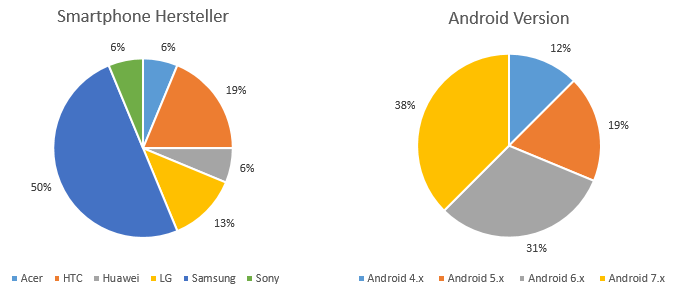
\includegraphics[width=\textwidth]{pics/SmartphoneAuswertung.png}
				\caption{Evaluation Auswertung - Die durchschnittliche Hard- und Software}
			\end{figure}
		
			Im folgenden Abschnitt dieses Kapitels wird nun das Ergebnis der Evaluation behandelt und ausgewertet. Der einzelnen Szenarien konnten von den Testern von "\-- -"\ bis "++" bewertet werden, während "++" die beste Bewertung darstellt. Damit das Ergebnis die Bewertung von allen Testern widerspiegelt, wurde "\-- -"\ mit -2 und "++" mit +2 verrechnet. Dies kann in Tabelle \ref{tab:ergbnisOverall} betrachtet werden. Diese entspricht dem des Bewertungsbogens, allerdings ohne nähere Beschreibung der einzelnen Szenarien. Die Punktzahl in der letzten Spalte spiegelt den genauen Durchschnitt von allen Testern wider.
			
			\begin{table}[htbp]
				\begin{tabular}{|l|l|c|c|c|c|c|c|}
					\hline
					\multirow{2}{*}{Szene} & \multirow{2}{*}{Szenario} &\multicolumn{5}{c}{Bewertung} \vline & \multirow{2}{*}{Punktzahl} \\ 
					& & -- & - & 0 & + & ++ & \\ \hline
					\multirow{3}{*}{Startscreen (Logged Out User)} & Log-In &  &  &  & x &  & 1,4 \\ 
					& Change Settings &  &  &  & x &  & 1,32 \\ 
					& Register &  &  &\multicolumn{2}{c}{x} \vline &  & 0,7 \\ \hline 
					\multirow{2}{*}{Registerszene} & Create new Account &  &  &  & x &  & 1,1 \\ 
					& Cancel Registration &  &  &  & x &  & 1 \\ \hline 
					\multirow{3}{*}{Startscreen (Logged In User)} & Log-In &  &  &  &\multicolumn{2}{c}{x} \vline & 1,6 \\ 
					& Log-Out &  &  &  & x &  & 1 \\ 
					& Change Settings &  &  &  & x &  & 1,3 \\ \hline 
					\multirow{10}{*}{Head Up Display} & Overview &  &  &  &\multicolumn{2}{c}{x} \vline & 1,6 \\  
					& Move Character &  &  &  & x &  & 1,4 \\  
					& Start Interaction &  &  &  & x &  & 1,3 \\  
					& Open Map &  &  &  &  & x & 1,7 \\  
					& Open Menu &  &  &  & x &  & 1,3 \\  
					& View Games &  &  &  &\multicolumn{2}{c}{x} \vline & 0,6 \\  
					& View Progress &  &  & x &  &  & 0,4 \\
					& View Achievements &  &  &  & x &  & 0,9 \\ 
					& Change Settings &  &  &  & x &  & 0,8 \\ 
					& Log-Out &  &  &  & x &  & 1 \\ 
					\hline
				\end{tabular}
				\caption{Ergebnis der Evaluation - Die Bewertung}
				\label{tab:ergbnisOverall}
			\end{table}
		
			Zunächst kann behauptet werden, dass die Auswertung positiv ausgefallen ist. Wenn alle Punkte von den einzelnen Szenarien zusammen betrachtet werden, ergibt es das Ergebnis von 1,1, welches in der Bewertungsmatrix unter "+" fallen würde.
			
			Positives aufzählen: Clean und Simple, wenig Text sondern mit Symbolen Aktion darstellen
			
			Häufige Punkte die angemerkt wurden - Register hervorheben, beim Abmelden erstmal warnen das man sich abmelden soll - dialog und nicht direkt und view games und progress besser gestalten - man merkt das es beim komplexen Informationen schwerer wird mit einfachen Gestaltungsprinzipien diese zu umzusetzen - Problem !

			Bewertung insgesamt - was fällt auf
			
			Auffällige - wenn man einzelne Gruppen betrachtet 
			
			Jüngere haben eher bei komplexeren wie registrierung oder view Progress schlechtere Bewertungen abgegeben, da diese Informationen eher weniger relevant war - schneller anfangen zu spielen nicht erst umständlich registriern 
			